\chapter{Eredmények, konklúzió}

\section{Az első tesztek}

Először is az implementált modell helyességét kell megvizsgálni. Ehhez vegyük szemügyre \aref{fig:cont_run}. ábrát. Láthatjuk rajta a három bejövő fázis áramát, illetve a DC feszültséget. A látottakról elmondható, hogy a görbék jellegüket tekintve helyesek, a kezdeti tranziens után állandósult állapotba kerül a rendszer. Az egyes fázisok áramai szimmetrikusak, az áram alakon, valamint a feszültség hullámosságon is megfigyelhető a várt, $50 Hz$-es hálózatból adódó $300\ Hz$-es hullámosság. A szimuláció $11\ A$-es konstans terhelés mellett készült, így jelentős $40\ V$-os DC hullámosság figyelhető meg.

\begin{figure}[H]
	\centering
	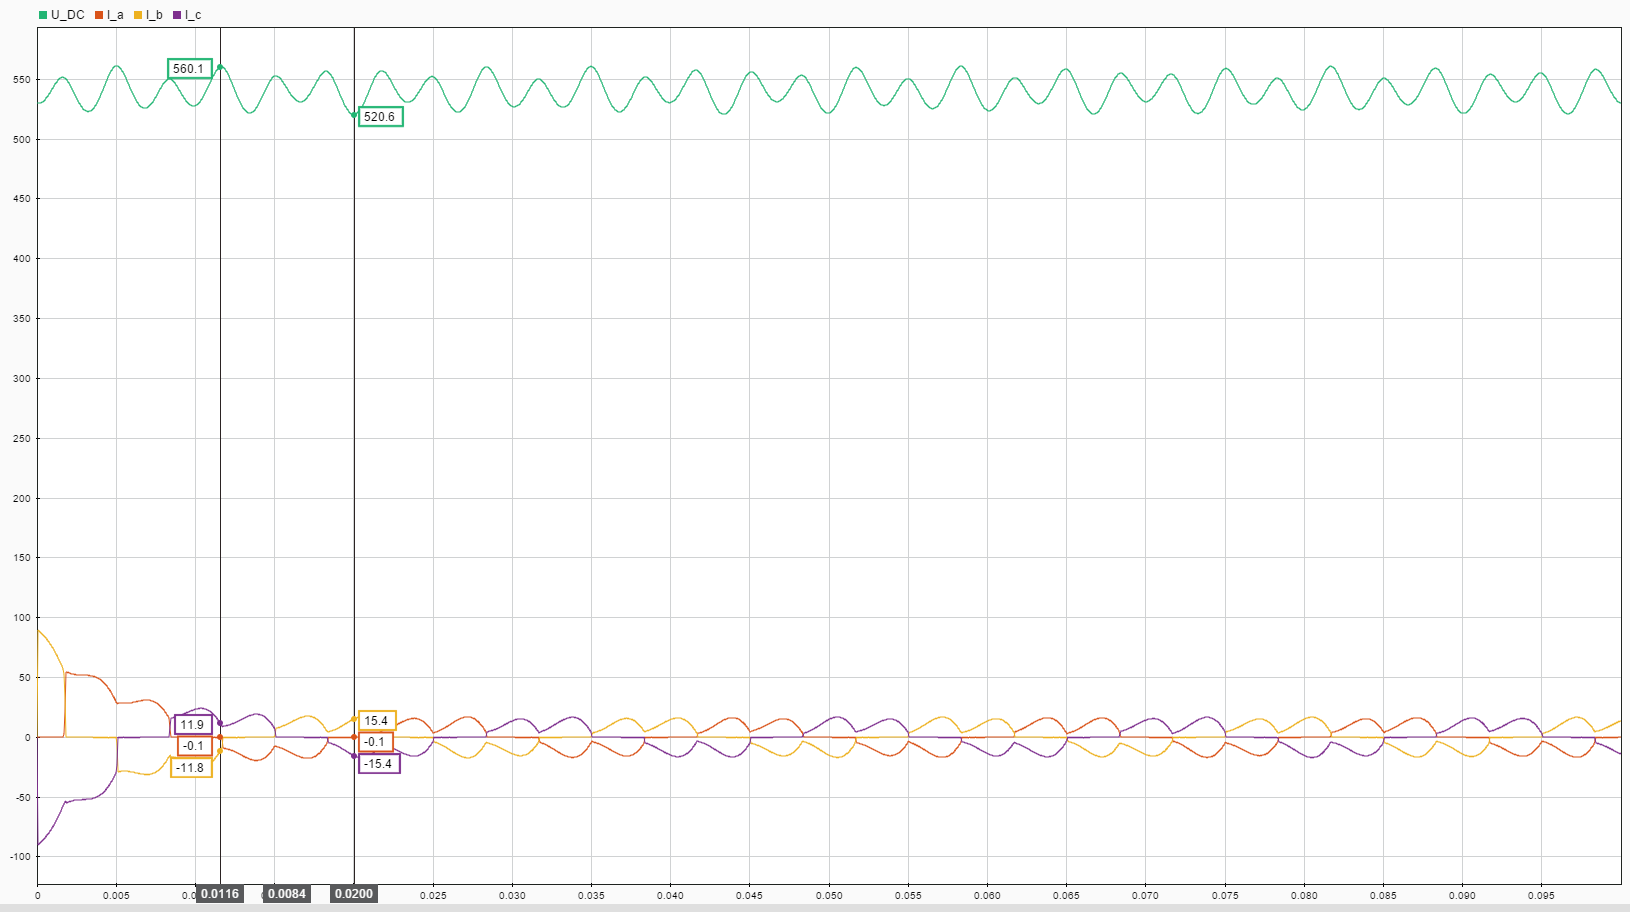
\includegraphics[width = \textwidth]{figures/continous_testrun_1.png}
	\caption{A szimuláció eredménye} 
	\label{fig:cont_run}
\end{figure}

\Aref{fig:meas_1}. ábrán már egy valós futás eredményét látjuk, a piros görbe a DC feszültség. Ez a mérés nem műszerrel készült, a frekvenciaváltó valós mérése került rögzítésre a HiTerm szoftver segítésgével. Láthatjuk, hogy a jelelek középértéke mintegy $30\ V$-al kisebb, ez a különbség a hálózat csúcsfeszültségének értékéből adódik. Szintén láthatjuk, hogy a kimenő áram csúcsértéke $16\ A$, melynek effektív értéke $\frac{16}{\sqrt{s}} \approx 11\ A$, így a szimuláció és a mérés eredménye összehasonlítható, hiszen a szimulált eszköz valódi példányán készült, hasonló futási paraméterek mellett. Láthatjuk, hogy a DC feszültség hullámossága ebben az esetben csak $30\ V$, ami jelentős eltérésnek tűnhet a szimulációval szemben, ennek azonban van magyarázata. A DC-link kondenzátor két sorba kötött B43544B5277M002 típusú elektrolit kondenzátor. Az alumínium-elektrolit kondenzátoroknak jellemzően nagy szórásuk van kapacitás tekintetében, az adatlapból leolvashatjuk, hgy ennek a konrét példánynak $\pm 20\%$, tehát a névleges érétktől valóban jelentősen eltréhet a valós kapacitás, aminek közveteln hatása van a mért DC hullámosságra.

\begin{figure}[H]
	\centering
	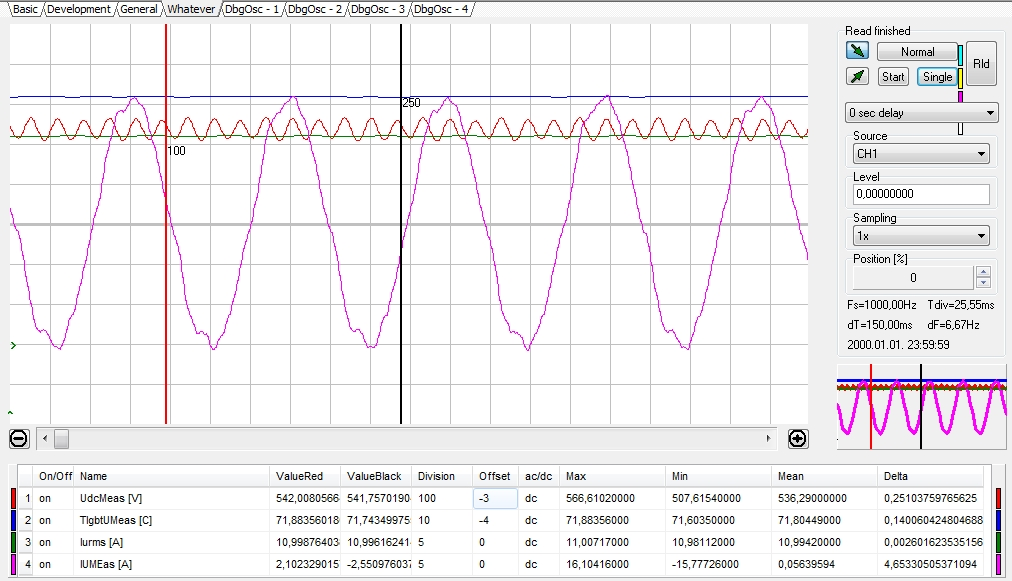
\includegraphics[width = \textwidth]{figures/50Hz_400V_LD12A_10k.jpeg}
	\caption{Egy valós mérés eredménye} 
	\label{fig:meas_1}
\end{figure}

\Aref{fig:hil_desk}. ábrán a teszteket megvalósító hardvert láthatjuk működés közben. Jól megfigyelhető, hogy bár nem az aktuális tervek szerinti hardvert láthatjuk, számos módosítás elvégzésre került rajta, hogy megfeledjen a követelményeknek, illetve hogy ki lehessen próbálni a módosítások hatását.

\begin{figure}[H]
	\centering
	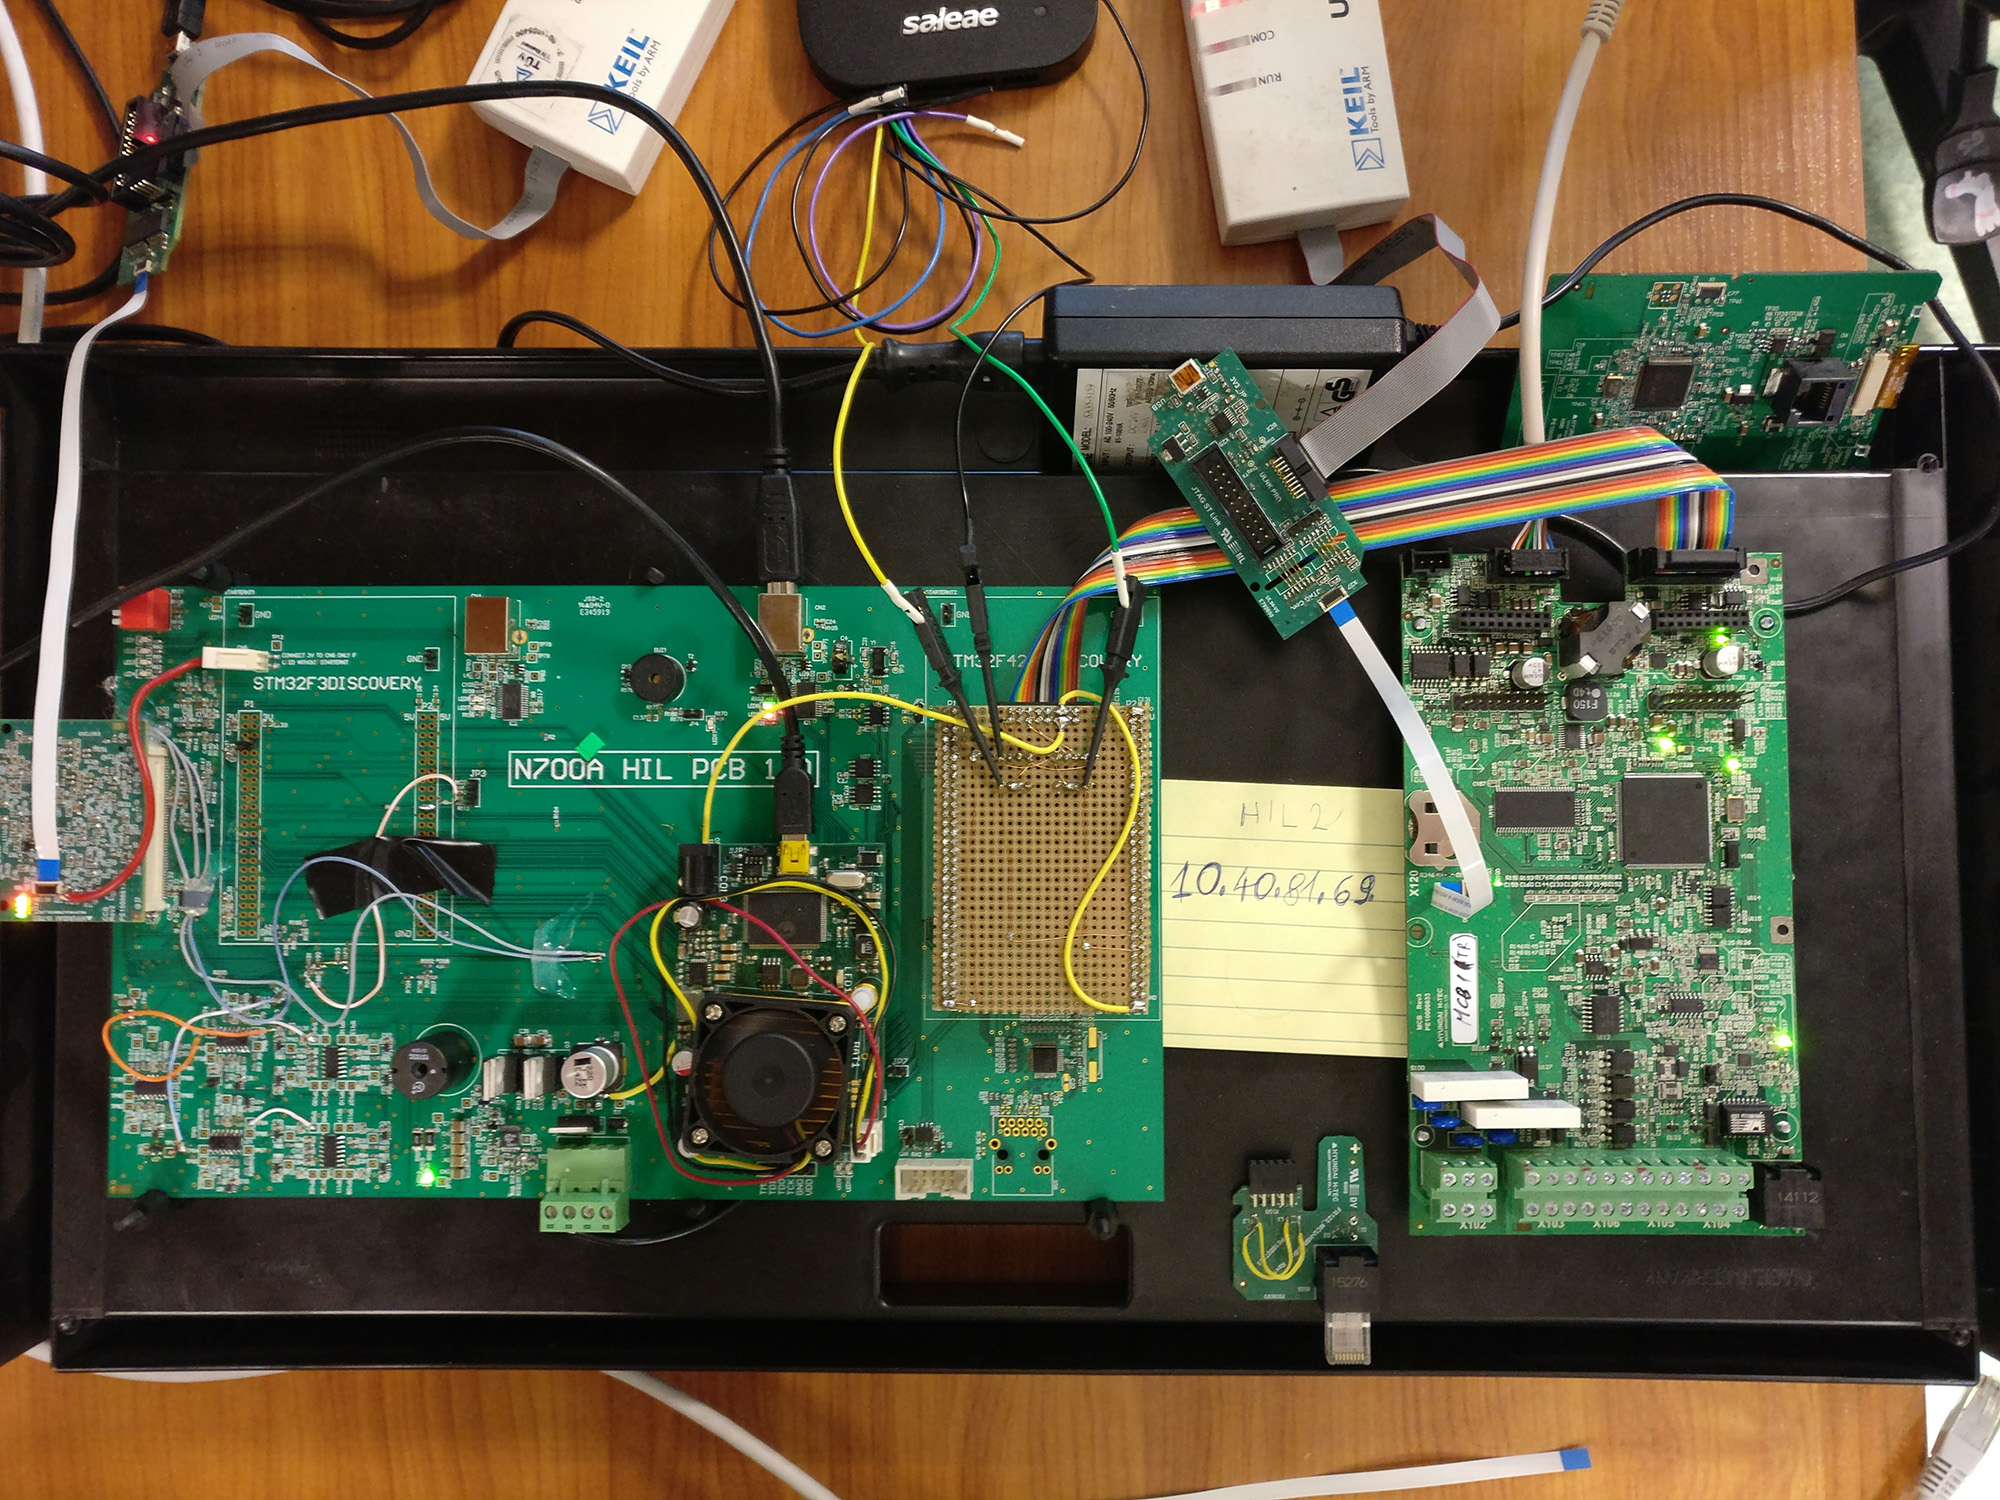
\includegraphics[width = \textwidth]{figures/hil_table.jpg}
	\caption{Az összeállított HIL deszkamodell} 
	\label{fig:hil_desk}
\end{figure}

\Aref{fig:office_testbench}. ábárán látható az úgynevezett ,,office testbench''
 azaz az irodai tesztpadunk. Erre fel van szerelve két egymásnak fordított $1,1\ kW$-os motor, az egyiket a Hyundai által fejlesztett Frame 1-es frekvenciaváltó hajtja, a másikat egy PROCON gyártmányú. Az eszköz segítségével könnyedén ki tudjuk próbálni a szoftver módosításait a nagy áramú laboratórium segítsége nélkül, tetszőleges terhelés mellett. 

\begin{figure}[H]
	\centering
	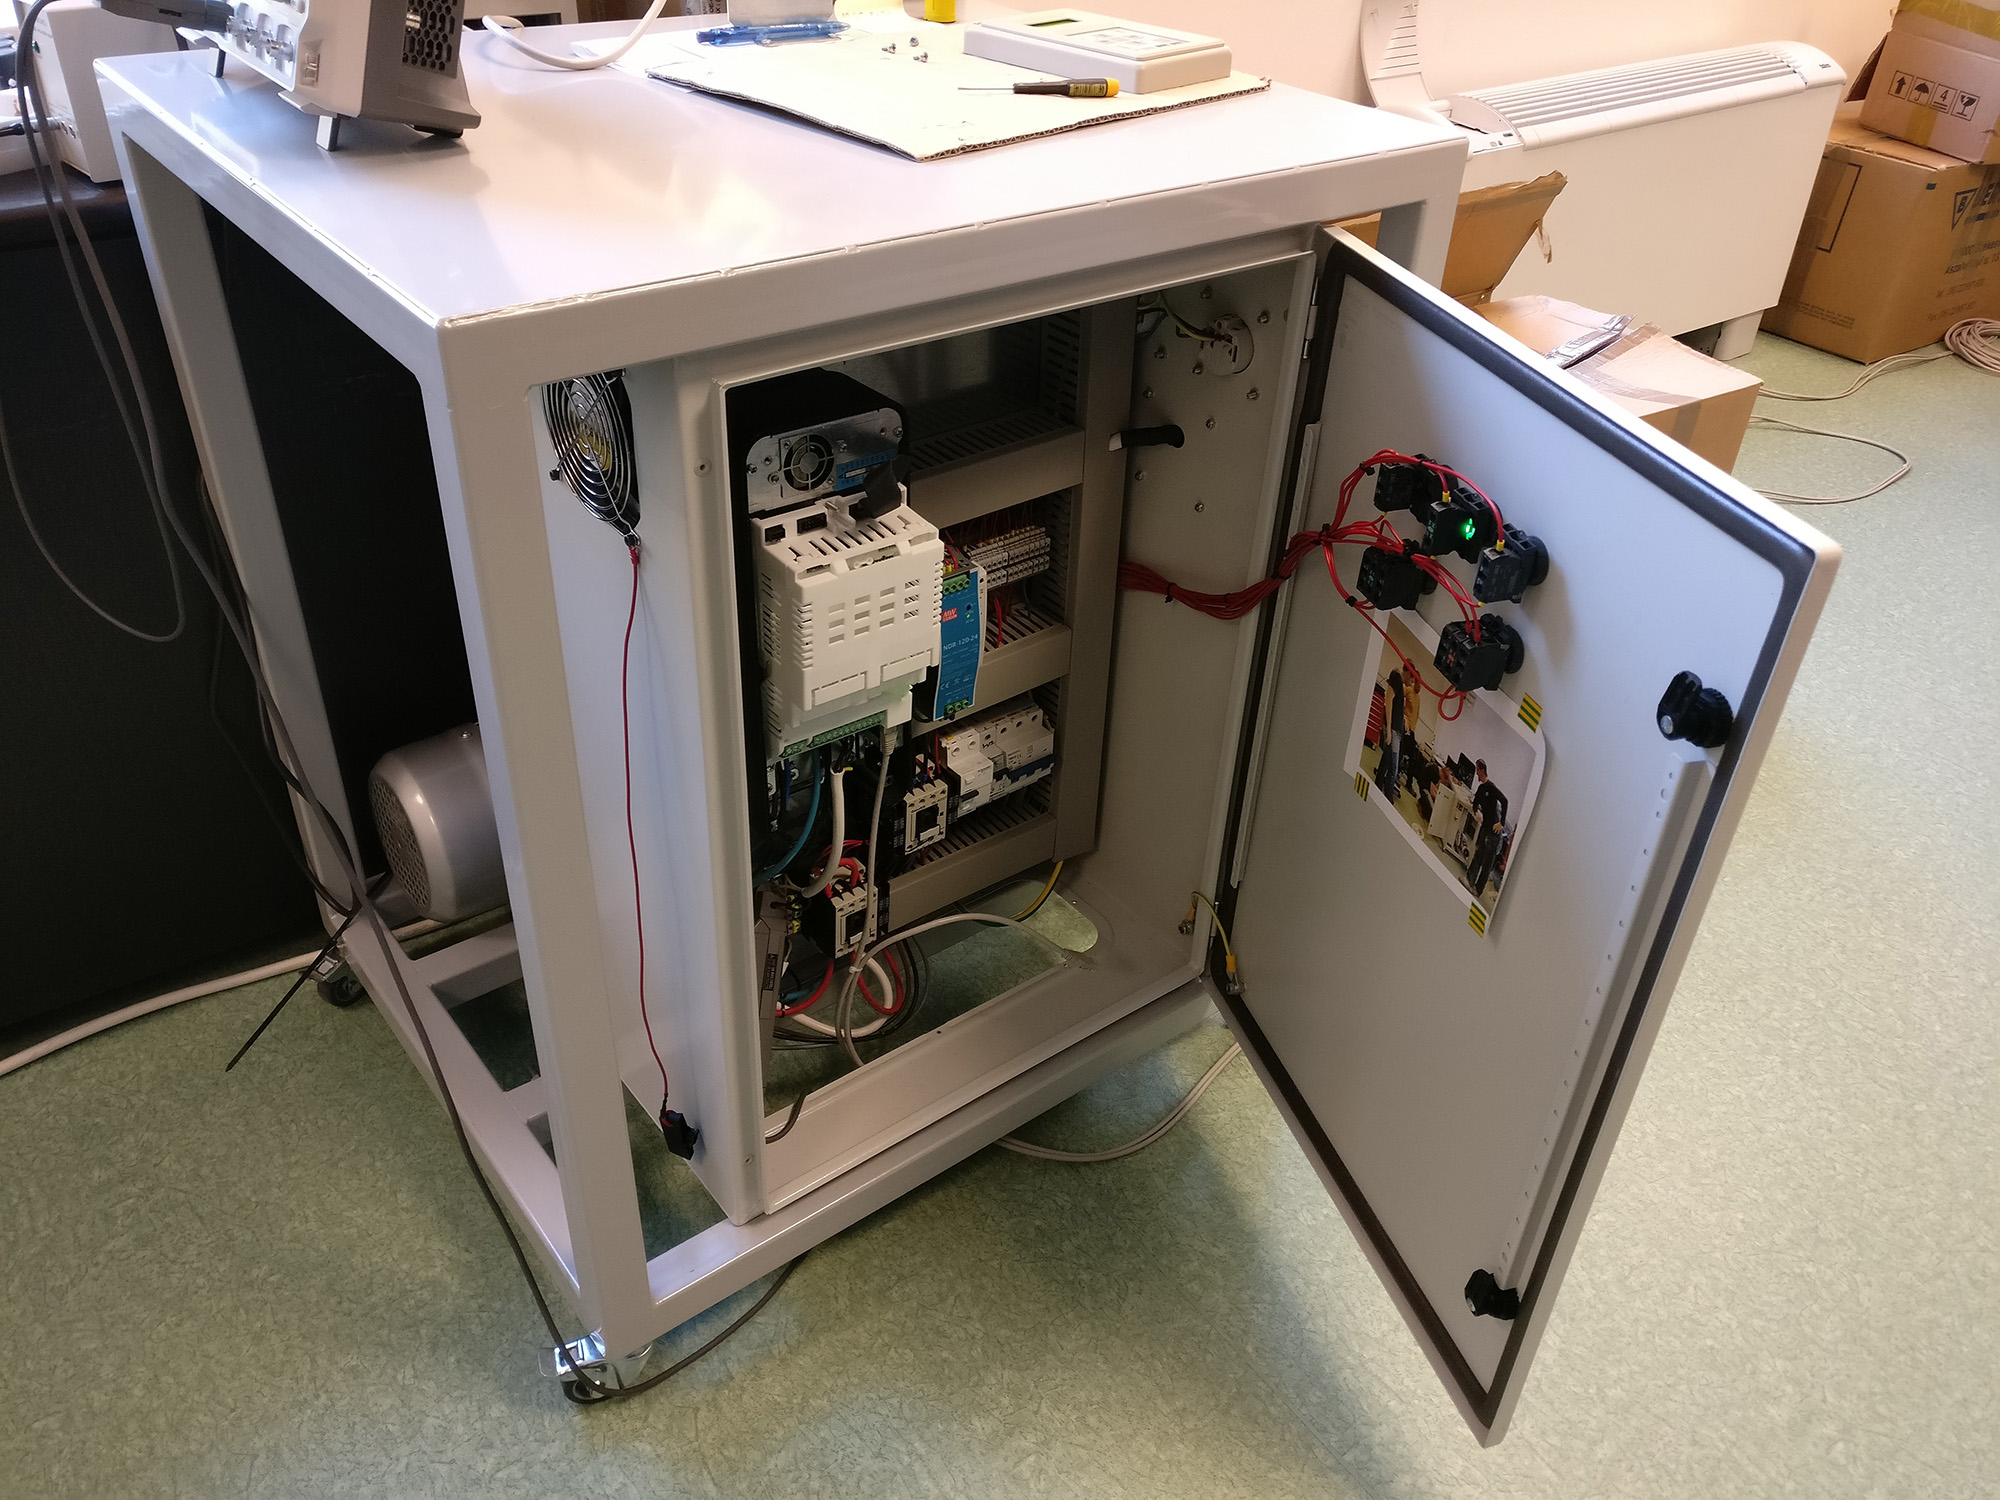
\includegraphics[width = \textwidth]{figures/office_testbench.jpg}
	\caption{Az ,,office testbench''} 
	\label{fig:office_testbench}
\end{figure}



\section{Konklúzió}

A dolgozat írása idején új hardver még nem készült el, a régin azonban el lettek végezve azokat a módosítások, melyek a jövőben gyártásba fognak kerülni. A jelenleg készített modellt így ki lehet próbálni, reprezentatív méréseket lehet rajta végezni.

A HIL-ben jelenleg a Frame 1 paraméterei szerinti modell található, ami jelen esetben különösen szerencsés, mert Frame 1-ből rendelkezésre áll egy laborban tesztelhető példány így a szimuláció közvetlenül összehasonlítható a valósággal.



\section{További lehetőségek}

Mint ahogy azt korábban is írtam, a téma még számos továbbfejlesztési lehetőséget tartogat magában. A bemeneti modellen lehet még fejleszteni, hogy valóban minden lehetséges üzemállapotot szimulálni tudjunk. A jelenlegi konfiguráció a funkcionális tesztekhez elegendő, de még pontosabb teszteket tudunk végezni egy a valósághoz közelebb álló modellel.

Ezen felül látok még fejlődési lehetőséget magában a keretrendszerben is. A Vivado már támogat grafikus tervezést verilog szinten is, az egyes IP-k elérhetőek a Simulinkhez hasonló környezetben is, így a megfelelő összeköttetéseket grafikusan biztosítva. Természetesen a funkcionalitás leírását nem kerülhetjük el, azonban egy jobban áttekinthető és könnyebben szerkeszthető rendszert kapunk ilyen módon. Azt szeretném elérni, hogy a MATLAB által generált modul elérhető legyen ilyen formában is, felgyorsítva ezzel a fejlesztést.